% !TEX program = xelatex
\documentclass[tikz]{standalone}
\usepackage{ctex}
\usepackage{fontawesome}
\usepackage{tikz}
\usepackage{epstopdf}
\usetikzlibrary{arrows,decorations.markings}
\usetikzlibrary{decorations.pathreplacing}
\usetikzlibrary{calc}
\definecolor{babypink}{rgb}{0.96, 0.76, 0.76}
\definecolor{babyblue}{rgb}{0.54, 0.81, 0.94}
\definecolor{cadmiumgreen}{rgb}{0.0, 0.42, 0.24}

\begin{document}

  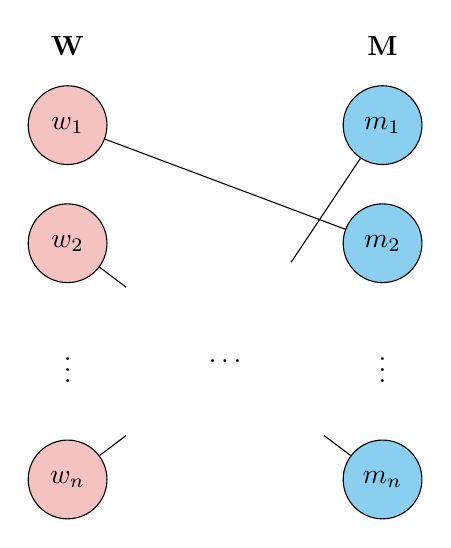
\begin{tikzpicture}[decoration={
      markings,
      mark=at position 1 with {\arrow[scale=1]{angle 90}};
    }]
    \path (0,1) node {$\mathbf{W}$};
\node[circle,draw,fill=babypink,minimum size=1cm] (w1) at (0,0) {$w_1$};
\node[circle,draw,fill=babypink,minimum size=1cm] (w2) at (0,-1.5) {$w_2$};
\path (0,-3) node {$ \vdots $};
\node[circle,draw,fill=babypink,minimum size=1cm] (wn) at (0,-4.5) {$w_n$};


\path (4,1) node {$\mathbf{M}$};
\node[circle,draw,fill=babyblue,minimum size=1cm] (m1) at (4,0) {$m_1$};
\node[circle,draw,fill=babyblue,minimum size=1cm] (m2) at (4,-1.5) {$m_2$};
\path (4,-3) node {$ \vdots $};
\node[circle,draw,fill=babyblue,minimum size=1cm] (mn) at (4,-4.5) {$m_n$};
\node[rectangle,minimum size=2.5cm] (c) at (2,-3) {$\ldots$};

\draw (w1)--(m2);
\draw (w2)--(c);
\draw (m1)--(c);
\draw (wn)--(c);
\draw (mn)--(c);

  \end{tikzpicture}
  
  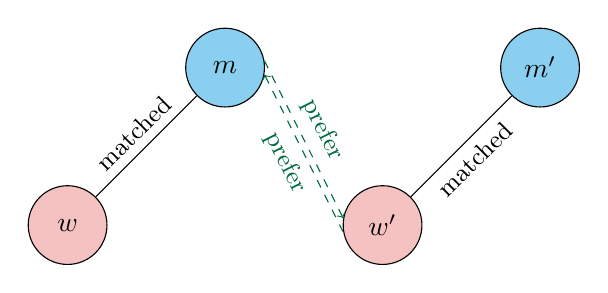
\begin{tikzpicture}[decoration={
      markings,
      mark=at position 1 with {\arrow[scale=1]{angle 90}};
    }]

    \node[circle,draw,fill=babypink,minimum size=1cm] (w1) at (0,0) {$w$};
\node[circle,draw,fill=babyblue,minimum size=1cm] (m1) at (2,2) {$m$};
\node[circle,draw,fill=babypink,minimum size=1cm] (w2) at (4,0) {$w'$};
\node[circle,draw,fill=babyblue,minimum size=1cm] (m2) at (6,2) {$m'$};
\draw (w1) -- node[sloped,above]{\small matched} (m1) ;
\draw (w2) -- node[sloped,below]{\small matched} (m2) ;
\draw[dashed,color=cadmiumgreen,->] (m1.10) --node[sloped,above]{\small prefer} (w2.170);
\draw[dashed,color=cadmiumgreen,->] (w2.190) --node[sloped,below]{\small prefer} (m1.350);


  \end{tikzpicture}
\end{document}
